\documentclass[11pt]{article}

% ---- Template settings: DO NOT change font size, margins or line spacing ----
\usepackage[margin=1in]{geometry}
\usepackage{amsmath,amssymb}
\usepackage{array}
\usepackage{booktabs}
\usepackage{enumitem}
\usepackage{xcolor}
\usepackage{hyperref}
\usepackage{setspace}
% ---- Added packages (do not affect page geometry) ----
\usepackage{graphicx}
\usepackage{multirow}
\usepackage{longtable}
\usepackage{caption}
\captionsetup{font=small,labelfont=bf,skip=4pt}

\setstretch{1.10}
\setlength{\emergencystretch}{2em}

\hypersetup{
    colorlinks=true,
    linkcolor=blue!50!black,
    urlcolor=blue!50!black,
    citecolor=black
}

% TODO marker: shows up in red in the PDF so nothing is forgotten.
% Before submission: grep -rn "\\todo" sections/ must return nothing.
\newcommand{\todo}[1]{\leavevmode{\color{red}\small[TODO: #1]}}
% Condition labels, keep consistent across sections
\newcommand{\condA}{\textsf{A}}
\newcommand{\condB}{\textsf{B}}
\newcommand{\condC}{\textsf{C}}
\newcommand{\condD}{\textsf{D}}

% --------------------
% Course information
% --------------------
\newcommand{\course}{DSA4213: Natural Language Processing for Data Science}
\newcommand{\semester}{Semester 1, AY2026/2027}

\begin{document}

\begin{center}
{\LARGE\bfseries Group Project Final Report}\\[0.4em]
{\large Improving Repository Navigation and Bug Localization in Minimal Software Engineering Agents}\\[0.9em]
Group ID: \underline{25}\\[0.9em]
\course\\
\semester
\end{center}

% ==================== MAIN TEXT (strict 8-page limit) ====================
% =====================================================================
% Owner: editor (3)   Budget: ~0.5 page   Source: slide 1, slide 16
% Write the Summary LAST, after §5 and §6 are final.
% =====================================================================
\section*{Administrative Information}

\begin{tabular}{@{}>{\bfseries\raggedright\arraybackslash}p{0.25\linewidth}
                    >{\raggedright\arraybackslash}p{0.70\linewidth}@{}}
Group members & Zhang Yuhang (A0351628B), Wang Chi (A0357310M), Chen Wenwen (A0351705J),
                Jiang Zhangzhang (A0355183B), Chen Xingyu (A0355370E) \\[0.7em]
Project direction & Software engineering agents: repository navigation and bug localization. \\[0.7em]
Repository & \url{https://github.com/235559649/DSA4213_group_work} \\
\end{tabular}

\section*{Project Summary}

% One paragraph, ~150 words. Must cover: question -> what we built -> how evaluated -> main findings.
% Main findings to state (keep the cautious tone of slide 10/16):
%  - 40 held-out SWE-bench Verified tasks, 4 conditions, 224 runs, gpt-5.4-mini.
%  - No hint hurt repair; C resolved most (25/40 vs A 20/40), but within noise (McNemar p=0.13).
%  - Hints let the agent read the reference file at call 1: C 30/40 vs A 6/40.
%  - 60 of 71 failures happened after the reference file was opened -> fixing, not finding, is the bottleneck.
%  - Failure feedback fired in 10/40 D runs and moved a reference file up once.
\todo{Summary paragraph (write last).}
   % owner: editor (3)      ~0.5 p
% =====================================================================
% Owner: 3   Budget: ~0.6 page   Source: slide 2, proposal §1
% =====================================================================
\section*{1. Problem, Research Question, and Motivation}

% Para 1 - Problem: issues describe symptoms, not files; a Django checkout has ~2,700 .py files
%   and ~38,000 indexed entities while the reference fix touches 1-3 files (slide 2).
%   mini-SWE-agent explores blindly with grep/find/cat; tracebacks from its own failed runs
%   are never used to re-prioritise.
% Para 2 - Why agent-based: debugging is iterative; inspection and execution produce the evidence
%   for the next action. Intended users: maintainers of Python repositories.
\todo{Problem and motivation (2 short paragraphs).}

% RQs: copy wording from proposal §1.1-1.2 (shortened). Keep the labels RQ1-RQ3 -
% §5 and §6 refer back to them.
\begin{itemize}[leftmargin=*,itemsep=0.1em,topsep=0.2em]
  \item \textbf{RQ1 (repair).} Can structured repository navigation and runtime failure evidence
        help mini-SWE-agent localize relevant code more efficiently without reducing bug-fixing success?
  \item \textbf{RQ2 (cost).} Does improved localization reduce exploration cost (files inspected,
        model steps, tokens, runtime) after accounting for localization overhead?
  \item \textbf{RQ3 (signal).} What do repository structure and runtime failure evidence add
        beyond textual issue-to-code relevance?
\end{itemize}

% Success definition (proposal §1.3): better localization + better repair, OR comparable repair
% at lower exploration cost. Localization alone does not count as success.
\todo{Definition of success (2 sentences).}

\paragraph{Changes since the proposal.}
% Template asks for 2-3 sentences. Cover ALL of these, compactly:
%  - held-out set 100 -> 40 tasks (cost/runtime from the pilot); 20 dev tasks unchanged;
%  - limits 50 steps / 30 min / 150k tokens -> 250 steps / $3 / 60 s per command;
%  - hint top-5 -> top-20 source files, plus top-3 related tests listed separately
%    (prompt policy source_only+related_tests_v1), because dev failures came after the right file was seen
%    and test files took 2.9 of the top-20 slots;
%  - structural ranking S puts the top-10 BM25 seeds first (chosen on the dev set; see §4.2).
\todo{2--3 sentences on deviations from the proposal.}
         % owner: 3               ~0.6 p
% =====================================================================
% Owner: 3   Budget: ~0.7 page   Source: proposal §2 + Table 1, slide 31
% Proposal Table 1 is too long for the main text: turn it into ~3 short paragraphs
% (or a 4-row compact table). All keys below exist in references.bib.
% =====================================================================
\section*{2. Related Work and Contribution}

% Agent framework: SWE-agent shows the agent-computer interface matters \cite{yang2024sweagent};
%   mini-SWE-agent is the minimal baseline we keep fixed \cite{minisweagent}. SWE-bench / Verified \cite{jimenez2024swebench,openai2024verified}.
% Textual & staged localization: BugLocator \cite{zhou2012buglocator}, Agentless \cite{xia2024agentless}, BM25 \cite{robertson2009bm25}.
% Structural navigation: LocAgent \cite{chen2025locagent}, CoSIL \cite{jiang2025cosil}, RepoNav \cite{chai2026reponav}, GraphLocator \cite{liu2025graphlocator}.
% Execution-informed: AutoCodeRover \cite{zhang2024autocoderover}, IssueExec \cite{liu2026issueexec}.
% Fusion: RRF \cite{cormack2009rrf}.
\todo{Related work, 3 short paragraphs.}

\paragraph{Our contribution.}
% Be explicit about what is OURS vs assembled (graders check this):
%  C1 Python AST repository index (files, classes, functions, imports) + BM25 / import-graph / RRF ranking;
%  C2 failure-aware refinement: traceback -> index entities -> rerank, with bounded routing
%     (rank_update / edit_recovery / diagnostic_only), staleness & environment-error filters;
%  C3 controlled 4-condition study on 40 held-out tasks with official harness, trajectory-level
%     localization metrics and a manual failure taxonomy.
% Also cite what we USE: mini-SWE-agent 2.4.6, SWE-bench harness 5.0.2, OpenRouter gpt-5.4-mini.
\todo{Contribution paragraph (C1--C3).}
         % owner: 3               ~0.7 p
% =====================================================================
% Owner: 1   Budget: ~0.8 page   Source: slide 7, slide 8, proposal §3
% =====================================================================
\section*{3. Agent and Task Setup}

Each SWE-bench Verified instance provides an issue description together with a repository checked out at the task-specific \texttt{base\_commit}. The agent operates inside the corresponding SWE-bench Docker environment and produces one final Git patch. We use mini-SWE-agent 2.4.6 with its bash tool and linear interaction history. At each step, the model selects a shell action, receives the resulting observation (standard output, standard error, and exit status), and decides the next action. The agent may inspect the repository freely but is not given the reference patch or the official \texttt{FAIL\_TO\_PASS}/\texttt{PASS\_TO\_PASS} labels during generation.

The same model, repair instructions, Docker environment, and execution budgets are used in all four conditions; only the repository-localization context differs. Condition \condA{} is the original agent without an added hint. Conditions \condB{} and \condC{} append a localization hint before the first model call, using BM25 and $\mathrm{RRF}(L,S)$ respectively. Condition \condD{} starts from the same context as \condC{} and may inject a bounded evidence update after a usable runtime failure. A run terminates when the agent submits a patch, reaches 250 model steps or the \$3 budget, exceeds the 60\,s command limit, or encounters an unrecoverable environment failure. The official SWE-bench harness is applied only after generation and therefore cannot influence the agent trajectory.

\begin{table}[h]
\centering
\small
\caption{Experimental setup (slide 8).}
\label{tab:setup}
\begin{tabular}{@{}ll@{}}
\toprule
Setting & Value \\
\midrule
Benchmark & SWE-bench Verified (rev \texttt{78f471bf}) \\
Development set & 20 tasks: Django 6, SymPy 6, Sphinx 4, pytest 4 \\
Held-out set & 40 tasks: Django 12, SymPy 12, Sphinx 10, pytest 6 \\
Runs & 160 main ($40 \times 4$) + 64 stability ($8$ tasks $\times 2$ rounds $\times 4$) \\
Agent & mini-SWE-agent 2.4.6, bash tool \\
Model & \texttt{openai/gpt-5.4-mini} via OpenRouter \\
Limits per run & 250 steps, \$3.00, 60\,s per command \\
Evaluation & official harness, \texttt{swebench} 5.0.2 \\
\midrule
\condA & no hint (original mini-SWE-agent) \\
\condB & top-20 source files from BM25 ranking $L$ \\
\condC & top-20 source files from $\mathrm{RRF}(L,S)$ \\
\condD & \condC{} + reranked evidence after usable runtime failures \\
\bottomrule
\end{tabular}
\end{table}

Localization hints are advisory rather than hard constraints: the agent may still inspect any repository file. The prompt presents up to 20 ranked source files and lists related tests separately, while the full ranking is retained for later evaluation. Appendix A.1 shows an actual Condition \condC{} localization hint and summarizes a failure-driven update under Condition \condD{}.           % owner: 1               ~0.8 p
% =====================================================================
% Owners: 2 (4.1-4.3), 4 (4.4)   Budget: ~1.4 pages incl. figure
% Source: slides 3-7, docs/architecture/*.md
% =====================================================================
\section*{4. System Design}

\begin{figure}[h]
\centering
% Owner 1: export slide 3 as PDF (crop) -> figures/architecture.pdf
\IfFileExists{figures/architecture.pdf}{%
  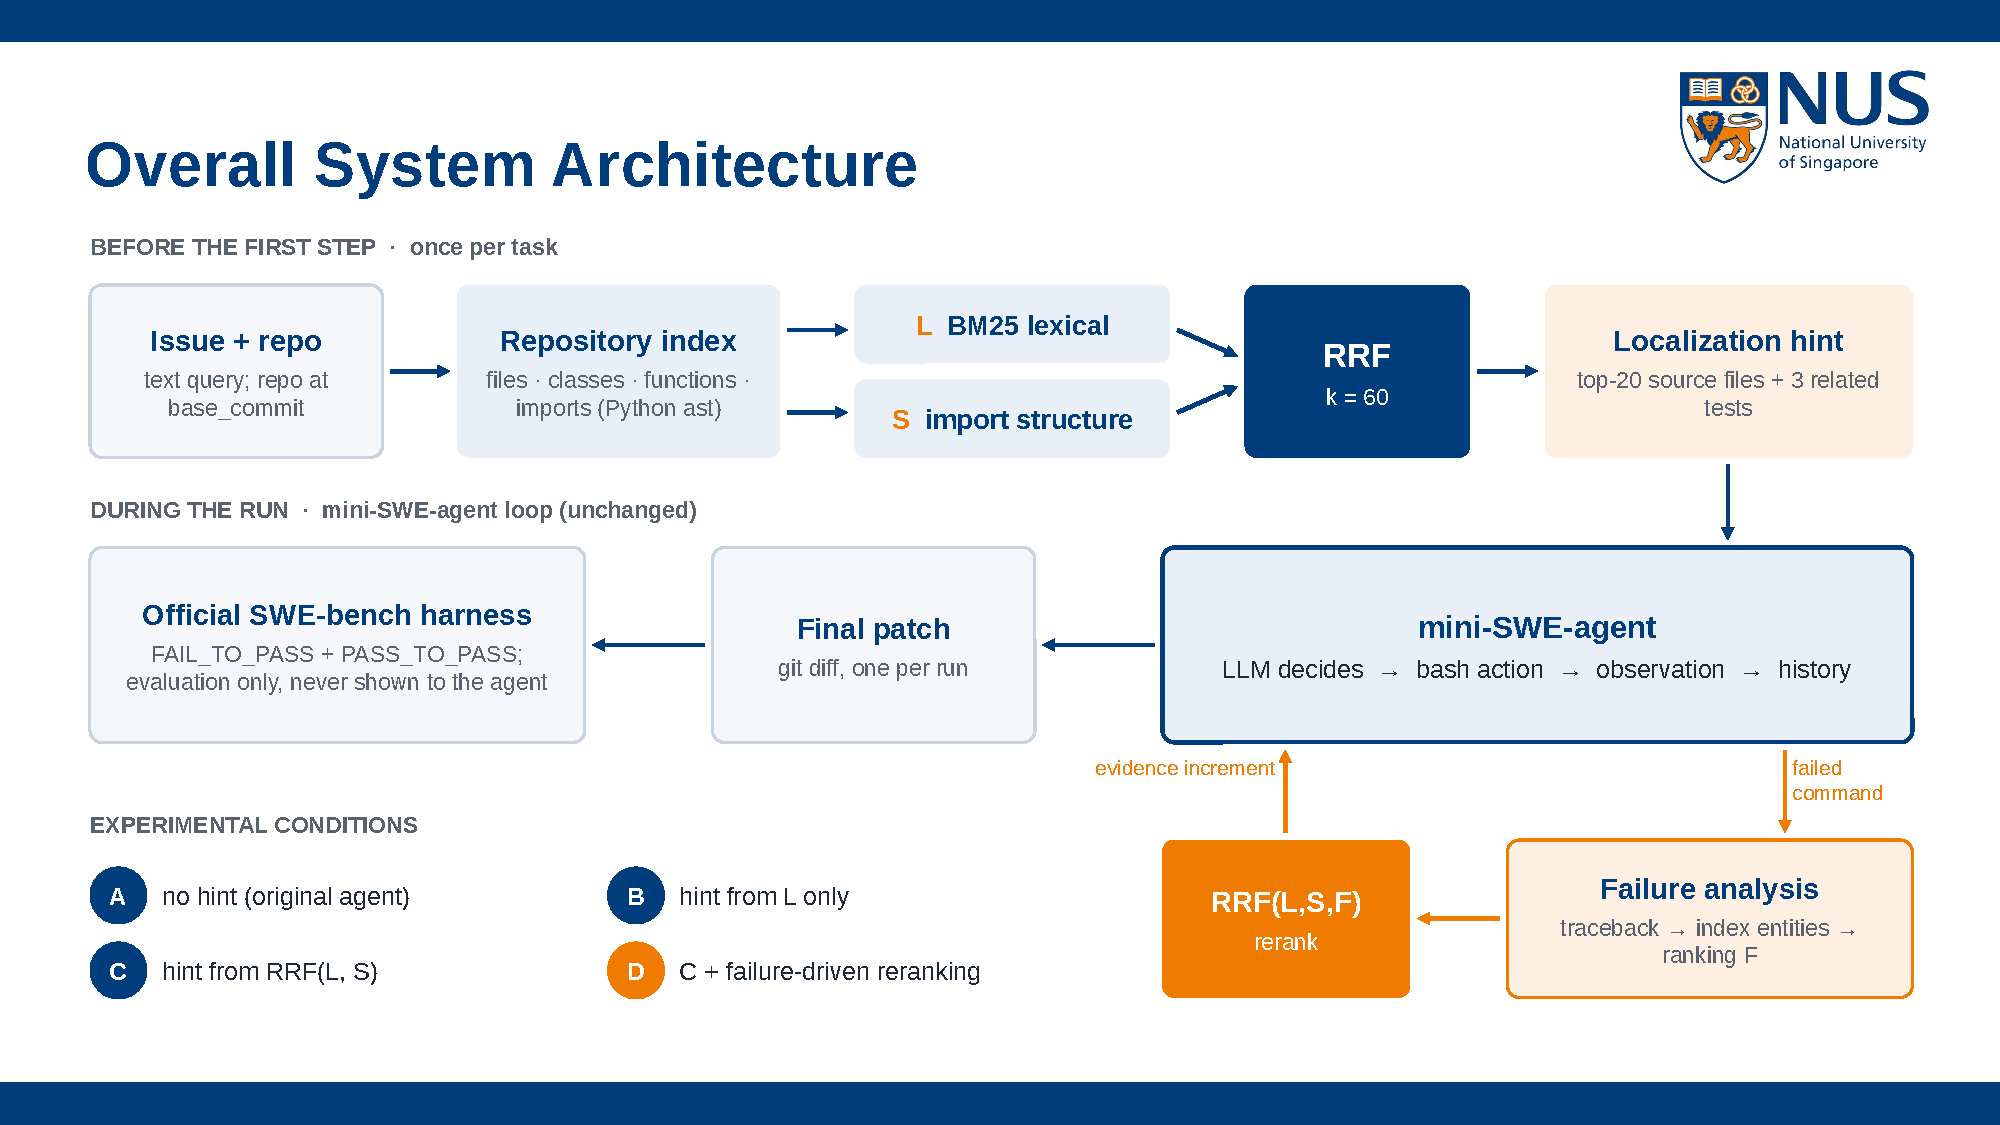
\includegraphics[width=\linewidth]{figures/architecture.pdf}%
}{%
  \fbox{\parbox[c][4.5cm][c]{0.9\linewidth}{\centering
  \todo{figures/architecture.pdf (export from slide 3)}}}%
}
\caption{System overview. The mini-SWE-agent loop is unchanged; \condB--\condD{} add a ranked
localization hint, and \condD{} reranks it when a failure yields usable evidence.}
\label{fig:arch}
\end{figure}

\subsection*{4.1 Repository index and lexical ranking}
% Owner 2. Implementation: src/repository/{ast_parser,indexer,swebench}.py, src/localization/keyword.py.
The index is the shared data layer for every condition. For each task we read every \texttt{.py}
file at the task's \texttt{base\_commit} directly from a git object store (no checkout), parse it
with Python's \texttt{ast} module, and store one record per module, class, function and method:
path, qualified symbol, line span, signature, docstring, and a retrieval text made of path, symbol
and source, truncated to 2,000 characters. Import statements are resolved to repository files,
giving each file $f$ a set of one-hop neighbours $N(f)$: the files it imports and the files that
import it. Files that fail to parse are recorded and skipped rather than aborting the build. On the
20 development tasks the index covers 27,484 files and 528,100 records; the only unparseable file
is a deliberate syntax-error fixture in Django's test suite. Building takes 0.4--13\,s per task and
is cached. In Condition~\condD{} the index is updated incrementally with the files the agent has
edited, so that traceback line numbers map to the right entities (Section~4.4).

The lexical ranking $L$ treats each record $e$ as a BM25 document~\cite{robertson2009bm25}, with
lower-cased identifier and number tokens, $k_1=1.5$ and $b=0.75$; the query is the issue text $q$.
A file takes the score of its best-matching entity,
\begin{equation*}
\mathrm{score}(e)=\sum_{t\in q}\mathrm{IDF}(t)\,
  \frac{\mathit{tf}_{t,e}\,(k_1+1)}{\mathit{tf}_{t,e}+k_1\bigl(1-b+b\,|e|/\mathit{avgdl}\bigr)},
\qquad
\mathrm{score}(f)=\max_{e\in f}\mathrm{score}(e),
\end{equation*}
so that one strongly matching function lifts its file while long files are not rewarded for
length alone. $L$ contains every file with a positive score (ties broken by path) and is the hint
source for Condition~\condB.

\subsection*{4.2 Structural ranking and RRF fusion}
% Owner 2. Implementation: src/localization/structural.py, src/localization/ranker.py.
The structural ranking $S$ uses the import graph to reach files the issue does not mention. The
seeds $Q$ are the top-10 files of $L$; each seed $q$ with lexical rank $r_L(q)$ shares a weight of
$1/r_L(q)$ equally among its non-test neighbours,
\begin{equation*}
s(f)=\sum_{q\in Q}\frac{\mathbf{1}[f\in N(q)]}{r_L(q)\,\max\bigl(1,|N(q)|\bigr)} .
\end{equation*}
$S$ lists the seeds first, in lexical order, followed by their neighbours in decreasing $s(f)$.
Condition~\condC{} fuses the two rankings with reciprocal rank fusion~\cite{cormack2009rrf},
$\mathrm{RRF}(f)=\sum_{r\in\{L,S\}}1/(60+r(f))$, where a file absent from a ranking contributes
nothing. RRF uses positions only, so BM25 scores and structural weights never need a common scale.

\paragraph{Design change from the proposal.} The proposal's $S$ contained only neighbours. In an
offline ablation on the development tasks (Appendix~A.2, Table~\ref{tab:dev-ablation}) that version
let files appearing in both lists overtake a correct file ranked first by BM25 alone
(django-11133: rank $1\to23$), lowering MRR from 0.500 to 0.393. Putting the seeds at the head of $S$
keeps $L$'s top~10 unchanged in $C$, so structure can only add files at ranks 11--20; this raised
Hit@20 from 0.75 to 0.85 with Hit@1, Hit@5 and MRR equal to or above $L$. The choice was made on
the development set before the held-out runs, so these numbers are optimistic; its effect on the
held-out tasks is reported in Section~5.1.

\subsection*{4.3 Prompt policy}
% Owner 2 (with 3). Implementation: src/agent/context.py (policy source_only+related_tests_v1).
In \condB--\condD{} the hint is appended once to the issue text before the first model call and is
labelled as navigation suggestions that the agent may ignore. It lists the top-20 \emph{source}
files of the condition's ranking, keeping their rank and score from the full ranking, and then, as
``possibly relevant existing tests'', the three highest-ranked test files of the same ranking
(an example is in Appendix~A.1). We adopted this policy after the development runs: most failures
there happened after the agent had already seen the right file, while test and documentation files
took on average 2.9 of the 20 slots. The source-file rule is the same one that defines the
evaluation targets (Section~5). The full, unfiltered ranking is logged for evaluation and is never
shown to the agent.

\subsection*{4.4 Failure-aware refinement (Condition D)}
% Owner 4. Source: slide 6. Wrap env.execute() and model.query().
% Pipeline: detect (exit status) -> parse (frames, exception, failing tests) -> map frames to index
% entities (index refreshed with edited files) -> rank F (nearest-to-exception first, 1/rank)
% -> RRF(L,S,F), w=1 -> short evidence note before next model call.
% Usability rules: >=1 frame maps to indexed source entity; setup errors never rerank;
% tests-only -> diagnostic note; stale workspace -> skipped; identical evidence not re-sent.
% Routing caps per run: rank_update 3, edit_recovery 2, diagnostic_only 1.
\todo{Failure-aware pipeline + usability rules (could be a 5-step list or pseudocode).}
          % owner: 2 (4.1-4.3), 4 (4.4)  ~1.4 p
% =====================================================================
% Owner: 5   Budget: ~2.0 pages
% Every number below was re-checked on 2026-11-09 against the final evidence
% package (DSA4213_final_20261028: official harness report.json per run,
% run_result.json, labels.json, prompt_candidates.json) and the Role 5
% analysis pages (tmp/claude-formal-charts-review-20261028).
% Per-run first-view data: data/first_reference_view.csv (from the Role 5 analysis page 06_exploration).
% =====================================================================
\section*{5. Evaluation and Results}

\paragraph{Protocol.}
All conditions ran on the same 40 held-out tasks with the same model, instructions, Docker images
and budgets; only the localization context differs (Table~\ref{tab:setup}). The proposal's primary
comparison is \condA{} vs \condD; \condB{} and \condC{} isolate the lexical and structural components.
\emph{Repair:} a run is resolved when the official harness~\cite{jimenez2024swebench,swebenchharness}
passes every \texttt{FAIL\_TO\_PASS} (F2P, target) and \texttt{PASS\_TO\_PASS} (P2P, existing) test.
Of the 224 runs, 216 were evaluated on the submitted patch; two (sympy-12489 \condB, \condC) were
re-evaluated on the original submission because the recorded patch file differed from it; and six
ended without a submission (e.g.\ repeated output-format errors) and were evaluated on the patch
extracted from their final state. Only one of the six passed (sympy-13757 \condB); counting all six as
unresolved changes \condB{} from 23 to 22 and nothing else.
\emph{Localization:} the usual file-level metrics~\cite{zhou2012buglocator,chen2025locagent}
(Hit@1/5/20, Recall@5, MRR) of the initial ranking, with the reference patch's Python source files as
targets (tests and documentation excluded; \condA{} has no ranking), plus the first model call whose
shell command reads a target file (\texttt{cat}, \texttt{sed}, \texttt{grep}, \dots; an approximation).
\emph{Efficiency:} model calls, tokens (including format-error retries), API cost and agent seconds;
ranking time is measured separately (Section~6).
\emph{Variability:} one main-round run per task and condition; 8 tasks, drawn before any result was
seen, ran two further rounds in every condition (64 runs). Paired differences use an exact McNemar test.

\begin{table}[h]
\centering\small
\caption{Main results on the 40 held-out tasks (one run per task and condition).
F2P = target tests; P2P = existing tests.}
\label{tab:main}
\begin{tabular}{@{}lcccc@{}}
\toprule
 & \condA{} original & \condB{} +text & \condC{} +structure & \condD{} +failures \\
\midrule
Resolved (/40)                          & 20 & 23 & \textbf{25} & 21 \\
F2P pass, P2P broken                    & 5  & 2  & 1  & 3  \\
F2P fail, P2P intact                    & 12 & 12 & 11 & 13 \\
F2P fail, P2P broken                    & 3  & 3  & 3  & 3  \\
\midrule
Reference file viewed at call 1 (/40)   & 6  & 29 & \textbf{30} & 29 \\
Model calls (total)                     & 367 & 357 & 343 & 367 \\
Total tokens (M)                        & 3.18 & 3.76 & 3.69 & 3.64 \\
Tokens per resolved task (k)            & 159 & 163 & \textbf{148} & 173 \\
Cost (\$) / cost per resolved task (\$) & 0.86 / 0.043 & 1.22$^*$ / 0.053 & 1.05 / 0.042 & 0.95 / 0.045 \\
Median agent seconds per run            & 19 & 17 & 16 & 19 \\
\bottomrule
\end{tabular}\\[2pt]
{\footnotesize $^*$One \condB{} run (sphinx-9229) has incomplete cost records, so \condB's cost is a lower bound; token counts are complete.}
\end{table}

\paragraph{RQ1: repair.}
No hint reduced repair: \condC{} resolved the most tasks (25/40), \condA{} the fewest (20/40), \condB{}
and \condD{} 23 and 21. The ordering rests on 7 \emph{swing} tasks, since 19 tasks were resolved in every
condition and 14 in none (Appendix~A.3). \condC{} resolved six tasks that \condA{} did not and \condA{} one
that \condC{} did not (exact McNemar $p=0.13$); the pre-specified \condA{} vs \condD{} split is 1 vs 2
($p=1.0$). Two observations place these gaps within run-to-run noise. On the 30 tasks where \condD's
feedback never fired, its prompt is identical to \condC's, yet 3 outcomes differ. In the stability
subset the order becomes \condD{} 17, \condB{} 15, \condC{} 15, \condA{} 14 of 24, and every condition
flips at least one task across rounds (Appendix~A.5). We therefore claim that the hints did not hurt
repair, not that any condition repairs better.

The conditions differ less in fixing the target than in what else they break. Target tests pass in
25, 25, 26 and 24 runs for \condA--\condD, but \condA{} breaks existing tests in 5 of them and \condC{} in 1.
In pytest-10081 both edit the same condition in \texttt{src/\_pytest/unittest.py}: \condA{} replaces the
skip check with one on the parent class and breaks 1 of 63 existing tests, while \condC{} keeps the
original check, adds the parent's and passes all 63. Passing the target tests is thus not the same as
a correct patch, a known risk in automated program repair~\cite{smith2015cure,yu2019overfitting}.
Whether structure causes fewer regressions is untested; we report it only as a lead.

\paragraph{RQ2: exploration cost.}
Hints bring a reference file into view about one model call earlier: at the first call the agent had
read one in 29--30 of 40 tasks with a hint and in 6 without, and by the second call \condA{} has caught
up (31 vs 31--34). The hint thus replaces the initial search, not later work. Hinted runs used more
tokens in total (3.64--3.76M vs 3.18M), because the ${\sim}550$-token hint stays in the history and is
re-sent with every call (5.5\% of input tokens). Per resolved task \condC{} was the cheapest (148k vs
159k for \condA), and on the six tasks only \condC{} solved it used 330k tokens to \condA's 454k. The
saving comes from harder tasks: on the 19 tasks every condition solved, the hint is pure overhead
(mean 55k vs 40k tokens per run for \condC{} vs \condA). Against the success criterion of Section~1,
\condC{} gives comparable repair at a lower cost \emph{per fix}, but not at a lower total cost.

\subsection*{5.1 Comparisons and Ablations}

\begin{table}[h]
\centering\small
\caption{Initial ranking quality on the 40 held-out tasks (counts of tasks unless stated); \condD's
initial ranking is identical to \condC's. ``In hint'': a target is among the 20 source files shown
(tests are filtered out first, so this can exceed Hit@20); ``Viewed'': the agent read a target, among
the Hit@20 tasks.}
\label{tab:loc}
\begin{tabular}{@{}lccccccc@{}}
\toprule
 & Hit@1 & Hit@5 & Recall@5 & MRR & Hit@20 & In hint & Viewed \\
\midrule
\condB{} (BM25 $L$)            & 9 & 16 & 38.8\% & 0.320 & 27 & 30 & 27/27 \\
\condC{} ($\mathrm{RRF}(L,S)$) & 9 & 16 & 38.8\% & 0.322 & 28 & 30 & 28/28 \\
\bottomrule
\end{tabular}
\end{table}

\paragraph{\condB{} vs \condC: what structure adds.}
\condC{} keeps \condB's top~10 (Section~4.2), so Hit@1 and Hit@5 are identical and MRR differs by 0.002.
Structure acts only on ranks 11--20, adding one task to Hit@20 (28 vs 27; Django $+2$, SymPy $-1$). The
clearest gain is django-16950: its reference file moves from rank 35 to 19 and enters \condC's hint;
both conditions resolved it, \condC{} with 62k tokens and \condB{} with 127k. On repair, \condC{} resolved
two tasks that \condB{} did not and never the reverse, too few to attribute to structure.

\paragraph{\condC{} vs \condD: what failure feedback adds.}
\condD{} resolved four tasks fewer than \condC{} and none that \condC{} missed (django-14311,
django-16950, sphinx-7757, pytest-7521). Feedback reached the agent in only one of these runs, and only
as a diagnostic note (django-14311), so the gap is mostly noise rather than an effect of feedback.
Overall, feedback was delivered in 10 of 40 \condD{} runs and re-ranked files in 5; Section~6 explains
why it rarely changed the outcome.
         % owner: 5               ~2.0 p
% =====================================================================
% Owner: 4 (costs paragraph: 5)   Budget: ~1.5 pages
% Source: slides 14, 15, 20, 21, 24, 16 (limitations), proposal §6
% =====================================================================
\section*{6. Analysis of Results, Failures, Limitations, Costs, and Risks}

\paragraph{The bottleneck is the fix, not the file.}

\begin{table}[h]
\centering\small
\caption{Main cause of the 71 unresolved main-round runs, assigned by reading each failed
patch against the official fix. No environment failures (F5) occurred.}
\label{tab:failures}
\begin{tabular}{@{}lccccc@{}}
\toprule
Failure class & \condA & \condB & \condC & \condD & All \\
\midrule
F1 never opened the reference file       & 2 & 3 & 3 & 3 & 11 \\
F2 opened it, misdiagnosed the cause     & 7 & 8 & 7 & 7 & 29 \\
F3 right location, incomplete fix        & 6 & 3 & 3 & 6 & 18 \\
F4 target fixed, existing tests broken   & 5 & 3 & 2 & 3 & 13 \\
\midrule
Unresolved                               & 20 & 17 & 15 & 19 & 71 \\
\bottomrule
\end{tabular}
\end{table}

% 60/71 failures came after the reference file was opened; F2 largest and flat across conditions (7-8);
% 12 of 29 F2 then edited a different file; 56/71 failures on the 14 tasks nobody solved.
% Case django-13590: all four conditions edit the same line as the official fix but break list/tuple
% lookups (P2P 140-144/145). => localization hints cannot help with "what to change".
% Mention who labelled the failures and how (one coder? second check?) - graders will ask.
\todo{Failure analysis paragraph + django-13590 case (3--4 sentences).}

\paragraph{Why failure feedback rarely helped (RQ3).}
% Funnel (slide 15): 52 candidate events in 23 D runs -> 15 messages delivered to 10 runs ->
% 5 first feedbacks re-ranked files -> 1 reference file moved up (sympy-18189: #2 -> #1; task solved by
% all conditions anyway). Held back: source unclear 12, weak signal 5, printed source 5, route limit 5,
% environment 5, other 5. All 5 re-ranks were in sympy.
% Interpretation: by the time the agent fails, it already has the right file; its failures are about
% what to change. Feedback added 95 s over 40 runs.
\todo{Failure-feedback funnel + interpretation.}

\paragraph{Costs.}
% Owner 5. T_loc vs T_agent definitions (docs/evaluation/timing.md). Index build 301 s for 40 tasks
% (83% of C's ranking time; sympy ~19 s/task); BM25 47 s; structure+RRF 12.5 s; per-task median B 5.6 s / C 6.0 s.
% 26 runs > 150k tokens used 47% of all tokens and resolved 2. Easy tasks: hint is overhead
% (A 40k vs C 55k per run); swing tasks: C cheapest (79k).
\todo{Cost paragraph (point to Table~\ref{tab:main} for totals).}

\paragraph{Limitations and risks.}
% - Small sample: 40 tasks, 4 repos, one model; stability on 8 tasks only; differences within noise.
% - Seeds-head S and prompt policy chosen on dev set.
% - Reference-patch files are imperfect localization targets (alternative fixes); tests != correctness.
% - Benchmark contamination (public issues in training data).
% - Structure-vs-regressions link is untested (mechanism).
% - Risks: patches need human review; hints can misdirect (sphinx-7757: C solved with a file outside every hint).
\todo{Limitations and risks (compact list).}
        % owner: 4 (+5 for costs) ~1.5 p
% =====================================================================
% Owner: 1   Budget: ~0.3 page
% =====================================================================
\section*{7. Reproducibility and Responsible Practice}

The implementation is version-controlled in the project repository, with dependencies pinned where required (\texttt{mini-swe-agent==2.4.6}) and API configuration supplied through environment variables rather than committed credentials. The experimental pipeline is exposed through scripts for BM25 retrieval, structural ranking, RRF fusion, agent execution, comparison, and SWE-bench evaluation. The held-out implementation was frozen before final evaluation, and all conditions used the same model and task-specific SWE-bench Docker environments. Docker images were prepared before formal attempts so that first-time image downloads were not confused with agent execution, while completed runs were recorded individually to support safe resumption after infrastructure interruptions; technical retries were kept distinct from experimental stability repeats.

Only public benchmark repositories are executed, each inside an isolated Docker container. Repository contents and tool outputs are treated as untrusted inputs, no API credentials are included in the released materials, and generated patches are evaluated by the official SWE-bench harness and should still receive human review before real-world use.

           % owner: 1               ~0.3 p
% =====================================================================
% Owner: editor (3)   Budget: ~0.2 page   Source: slide 16
% =====================================================================
\section*{8. Conclusion}

% 3 findings + 1 take-home (slide 16):
% 1. No hint hurt repair; C resolved most with fewest regressions, within noise.
% 2. File hints put the agent on relevant code sooner (call 1: C 30/40 vs A 6/40), cheaper per fix.
% 3. Complete fixes remain the bottleneck; failure feedback added little.
% Next: use structure for change-impact analysis and related-test selection.
\todo{Conclusion paragraph.}
      % owner: editor (3)      ~0.2 p
% ==================== End of main text ====================
\clearpage

% =====================================================================
% Fill in TOGETHER (all 5). Shares must sum to 100.
% =====================================================================
\section*{Contribution Statement}

\begin{center}
\begin{tabular}{@{}>{\raggedright\arraybackslash}p{0.28\linewidth}
                >{\raggedright\arraybackslash}p{0.52\linewidth}
                >{\centering\arraybackslash}p{0.12\linewidth}@{}}
\toprule
\textbf{Member (Student ID)} & \textbf{Main contributions} & \textbf{Share (\%)} \\
\midrule
Zhang Yuhang (A0351628B)     & \todo{} & \\
Wang Chi (A0357310M)         & \todo{} & \\
Chen Wenwen (A0351705J)      & \todo{} & \\
Jiang Zhangzhang (A0355183B) & \todo{} & \\
Chen Xingyu (A0355370E)      & \todo{} & \\
\midrule
\textbf{Total} & & \textbf{100} \\
\bottomrule
\end{tabular}
\end{center}


\bibliographystyle{plain}
\bibliography{references}

\appendix
% =====================================================================
% Appendix - not counted, graders not required to read it.
% Owners: A.1 1 (prompt/trace), A.2 2 (dev ablation), A.3-A.5 5, A.6 4
% Anything cut from the main text to meet 8 pages goes here.
% =====================================================================
\section*{Appendix}

\subsection*{A.1 Localization hint and example trajectory}
% Owner 1: full hint block for django-11133 (slide 7) in a verbatim environment, plus a short
% D trajectory excerpt (sympy-18189: RecursionError -> rerank note), slide 15 / A8.
\todo{Prompt hint example and one agent trace excerpt.}

\subsection*{A.2 Development-set localization ablation}
\begin{table}[h]
\centering\small
\caption{File-level ranking quality on the 20 development tasks (\texttt{docs/analysis/localization-ablation.md}).
$S_0$/$C_0$: structural ranking as defined in the proposal (seeds excluded); $C$: seeds-head $S$ as run.
$L'$, $C'$: restricted to source files, as shown in the prompt. Optimistic: $C$ was chosen on these tasks.}
\label{tab:dev-ablation}
\begin{tabular}{@{}lcccccc@{}}
\toprule
Variant & Hit@1 & Hit@5 & Recall@5 & MRR & Hit@10 & Hit@20 \\
\midrule
$L$: BM25 (\condB)              & 0.40 & 0.60 & 0.567 & 0.500 & 0.65 & 0.75 \\
$S_0$: structure only           & 0.05 & 0.20 & 0.200 & 0.142 & 0.45 & 0.50 \\
$C_0$: $\mathrm{RRF}(L,S_0)$     & 0.30 & 0.55 & 0.492 & 0.393 & 0.55 & 0.65 \\
$C$: $\mathrm{RRF}(L,S)$, as run & 0.40 & 0.60 & 0.567 & 0.504 & 0.65 & 0.85 \\
$L'$: source only               & 0.50 & 0.70 & 0.667 & 0.586 & 0.75 & 0.75 \\
$C'$: source only               & 0.50 & 0.70 & 0.667 & 0.591 & 0.75 & 0.85 \\
\bottomrule
\end{tabular}
\end{table}

\subsection*{A.3 Swing tasks}
\begin{table}[h]
\centering\small
\caption{The 7 tasks on which conditions disagree. \checkmark{} resolved; F3 target test still fails;
F4 target fixed but an existing test broken. Rank = first reference file in the initial ranking of \condB{} / \condC{}
(ranks $>20$ are outside the hint).}
\label{tab:swing}
\begin{tabular}{@{}lccccc>{\raggedright\arraybackslash}p{0.38\linewidth}@{}}
\toprule
Task & \condA & \condB & \condC & \condD & Rank \condB/\condC & What differed \\
\midrule
django-14311 & F4 & \checkmark & \checkmark & F4 & 5 / 5 & A, D fixed the target but broke 3 autoreload tests \\
django-16950 & F4 & \checkmark & \checkmark & F4 & 35 / 19 & structure moved the file into C's hint \\
sympy-18698  & \checkmark & F3 & F3 & F3 & 1 / 1 & only A fixed it \\
sphinx-7757  & F3 & F3 & \checkmark & F3 & 97 / 110 & C fixed a file outside every hint \\
sphinx-9320  & F3 & \checkmark & \checkmark & \checkmark & 1 / 1 & A changed a shared helper: incomplete \\
pytest-7521  & F4 & \checkmark & \checkmark & F3 & 19 / 15 & A broke 2 capture tests; D left target failing \\
pytest-10081 & F4 & F4 & \checkmark & \checkmark & 58 / 35 & A, B replaced the skip check; C, D kept it \\
\bottomrule
\end{tabular}
\end{table}

\subsection*{A.4 Per-task results}
{\small
\setlength{\tabcolsep}{4pt}
\begin{longtable}{@{}llccccrrrrc@{}}
\caption{Per-task outcomes on the 40 held-out tasks (slides 18--19). Pattern: all / none / swing.
Rank = best reference file in the initial ranking. $\bullet$ = \condD{} feedback fired.}
\label{tab:pertask}\\
\toprule
Task & Pattern & \condA & \condB & \condC & \condD & Rank \condB & Rank \condC & Tok \condA{} (k) & Tok \condC{} (k) & FB \\
\midrule
\endfirsthead
\toprule
Task & Pattern & \condA & \condB & \condC & \condD & Rank \condB & Rank \condC & Tok \condA{} (k) & Tok \condC{} (k) & FB \\
\midrule
\endhead
django-7530  & all   & \checkmark & \checkmark & \checkmark & \checkmark & 42 & 25 & 26 & 120 & \\
django-10914 & all   & \checkmark & \checkmark & \checkmark & \checkmark & 804 & 818 & 24 & 44 & \\
django-11119 & all   & \checkmark & \checkmark & \checkmark & \checkmark & 81 & 20 & 50 & 34 & \\
django-12276 & all   & \checkmark & \checkmark & \checkmark & \checkmark & 1 & 1 & 55 & 63 & \\
django-13212 & none  & F3 & F3 & F3 & F3 & 15 & 14 & 54 & 95 & $\bullet$ \\
django-13590 & none  & F4 & F4 & F4 & F4 & 4 & 4 & 15 & 31 & \\
django-14311 & swing & F4 & \checkmark & \checkmark & F4 & 5 & 5 & 76 & 52 & $\bullet$ \\
django-15380 & all   & \checkmark & \checkmark & \checkmark & \checkmark & 2 & 2 & 56 & 23 & \\
django-16255 & all   & \checkmark & \checkmark & \checkmark & \checkmark & 1 & 1 & 27 & 31 & \\
django-16315 & none  & F3+4 & F3+4 & F3+4 & F3+4 & 3 & 3 & 60 & 112 & \\
django-16877 & all   & \checkmark & \checkmark & \checkmark & \checkmark & 1 & 1 & 26 & 42 & \\
django-16950 & swing & F4 & \checkmark & \checkmark & F4 & 35 & 19 & 99 & 62 & \\
sympy-12489  & none  & F3 & F3+4 & F3+4 & F3 & 3 & 3 & 34 & 90 & \\
sympy-13372  & all   & \checkmark & \checkmark & \checkmark & \checkmark & 1 & 1 & 35 & 22 & $\bullet$ \\
sympy-13757  & all   & \checkmark & \checkmark & \checkmark & \checkmark & 2 & 2 & 81 & 37 & \\
sympy-16886  & all   & \checkmark & \checkmark & \checkmark & \checkmark & 1 & 1 & 12 & 17 & \\
sympy-18189  & all   & \checkmark & \checkmark & \checkmark & \checkmark & 2 & 2 & 72 & 71 & $\bullet$ \\
sympy-18199  & none  & F3 & F3 & F3 & F3 & 6 & 6 & 57 & 41 & \\
sympy-18698  & swing & \checkmark & F3 & F3 & F3 & 1 & 1 & 215 & 226 & \\
sympy-19637  & all   & \checkmark & \checkmark & \checkmark & \checkmark & 1 & 1 & 18 & 30 & $\bullet$ \\
sympy-20428  & none  & F3 & F3 & F3 & F3 & 555 & 341 & 89 & 71 & $\bullet$ \\
sympy-21930  & none  & F3 & F3 & F3 & F3 & 12 & 51 & 137 & 111 & \\
sympy-22080  & none  & F3+4 & F3 & F3+4 & F3+4 & 254 & 156 & 195 & 151 & \\
sympy-24443  & all   & \checkmark & \checkmark & \checkmark & \checkmark & 1 & 1 & 36 & 53 & $\bullet$ \\
sphinx-7748  & none  & F3 & F3 & F3 & F3+4 & 15 & 21 & 126 & 92 & $\bullet$ \\
sphinx-7757  & swing & F3 & F3 & \checkmark & F3 & 97 & 110 & 116 & 81 & \\
sphinx-8269  & all   & \checkmark & \checkmark & \checkmark & \checkmark & 24 & 51 & 26 & 46 & \\
sphinx-8475  & all   & \checkmark & \checkmark & \checkmark & \checkmark & 11 & 15 & 30 & 44 & \\
sphinx-9229  & none  & F3 & F3 & F3 & F3 & 11 & 12 & 151 & 791 & \\
sphinx-9258  & none  & F3 & F3 & F3 & F3 & 31 & 18 & 324 & 200 & \\
sphinx-9320  & swing & F3 & \checkmark & \checkmark & \checkmark & 1 & 1 & 37 & 23 & \\
sphinx-9591  & none  & F3 & F3 & F3 & F3 & 32 & 29 & 122 & 86 & \\
sphinx-9698  & all   & \checkmark & \checkmark & \checkmark & \checkmark & 62 & 37 & 27 & 40 & \\
sphinx-11445 & none  & F3+4 & F3+4 & F3 & F3 & 16 & 12 & 361 & 197 & \\
pytest-7236  & all   & \checkmark & \checkmark & \checkmark & \checkmark & 11 & 11 & 101 & 244 & $\bullet$ \\
pytest-7324  & none  & F3 & F3 & F3 & F3 & 10 & 10 & 26 & 30 & $\bullet$ \\
pytest-7521  & swing & F4 & \checkmark & \checkmark & F3 & 19 & 15 & 84 & 56 & \\
pytest-7982  & all   & \checkmark & \checkmark & \checkmark & \checkmark & 31 & 22 & 14 & 23 & \\
pytest-8399  & all   & \checkmark & \checkmark & \checkmark & \checkmark & 19 & 12 & 41 & 56 & \\
pytest-10081 & swing & F4 & F4 & \checkmark & \checkmark & 58 & 35 & 42 & 55 & \\
\bottomrule
\end{longtable}
}

\subsection*{A.5 Stability: 8 tasks $\times$ 3 rounds}
\begin{table}[h]
\centering\small
\caption{Repeated runs on 8 tasks chosen before results were seen (rounds 1\,/\,2\,/\,3).
$^*$ = \condD{} feedback fired in that run.}
\label{tab:stability}
\begin{tabular}{@{}lcccc@{}}
\toprule
Task & \condA & \condB & \condC & \condD \\
\midrule
django-16315 & \texttimes\,\texttimes\,\texttimes & \texttimes\,\texttimes\,\texttimes & \texttimes\,\texttimes\,\texttimes & \texttimes\,\texttimes\,\texttimes \\
django-16877 & \checkmark\,\checkmark\,\checkmark & \checkmark\,\checkmark\,\checkmark & \checkmark\,\checkmark\,\texttimes & \checkmark\,\checkmark\,\checkmark \\
pytest-10081 & \texttimes\,\checkmark\,\texttimes & \texttimes\,\checkmark\,\checkmark & \checkmark\,\checkmark\,\checkmark & \checkmark\,\checkmark$^*$\,\checkmark \\
pytest-7982  & \checkmark\,\checkmark\,\checkmark & \checkmark\,\checkmark\,\checkmark & \checkmark\,\checkmark\,\checkmark & \checkmark\,\checkmark\,\checkmark \\
sphinx-9258  & \texttimes\,\texttimes\,\texttimes & \texttimes\,\texttimes\,\texttimes & \texttimes\,\texttimes\,\texttimes & \texttimes\,\texttimes\,\texttimes \\
sphinx-9320  & \texttimes\,\checkmark\,\checkmark & \checkmark\,\checkmark\,\checkmark & \checkmark\,\checkmark\,\checkmark & \checkmark\,\checkmark\,\checkmark \\
sympy-18189  & \checkmark\,\checkmark\,\texttimes & \checkmark\,\checkmark\,\checkmark & \checkmark\,\checkmark\,\checkmark & \checkmark$^*$\,\checkmark\,\texttimes \\
sympy-24443  & \checkmark\,\checkmark\,\checkmark & \checkmark\,\texttimes\,\texttimes & \checkmark\,\texttimes\,\texttimes & \checkmark$^*$\,\checkmark$^*$\,\checkmark \\
\midrule
Resolved (/24)          & 14 & 15 & 15 & 17 \\
Solved in all 3 rounds (/8) & 3 & 4 & 4 & 5 \\
\bottomrule
\end{tabular}
\end{table}

\subsection*{A.6 Failure-feedback details and case studies}
% Owner 4: slide 23 table (events / runs / feedback / re-rank / resolved by repo and pattern)
% and the two A8 case studies (django-16950 for structure, sympy-18189 for feedback).
\todo{Failure-feedback breakdown table and case studies.}
        % owners: 2, 4, 5

\end{document}
